%=======================02-713 LaTeX template, following the 15-210 template==================
%
% You don't need to use LaTeX or this template, but you must turn your homework in as
% a typeset PDF somehow.
%
% How to use:
%    1. Update your information in section "A" below
%    2. Write your answers in section "B" below. Precede answers for all 
%       parts of a question with the command "\question{n}{desc}" where n is
%       the question number and "desc" is a short, one-line description of 
%       the problem. There is no need to restate the problem.
%    3. If a question has multiple parts, precede the answer to part x with the
%       command "\part{x}".
%    4. If a problem asks you to design an algorithm, use the commands
%       \algorithm, \correctness, \runtime to precede your discussion of the 
%       description of the algorithm, its correctness, and its running time, respectively.
%    5. You can include graphics by using the command \includegraphics{FILENAME}
%
\documentclass[11pt]{article}
\usepackage{amsmath,amssymb,amsthm,enumitem}
\usepackage{graphicx}
\usepackage[margin=1in]{geometry}
\usepackage{fancyhdr}
\graphicspath{./images/}
\newtheorem{theorem}{Theorem}
\setlength{\parindent}{0pt}
\setlength{\parskip}{5pt plus 1pt}
\setlength{\headheight}{13.6pt}
\newcommand\question[2]{\vspace{.25in}\hrule\textbf{#1}: #2\vspace{.5em}\hrule\vspace{.10in}}
\renewcommand\part[1]{\vspace{.10in}(#1)\par}
\newcommand\algorithm{\vspace{.10in}\textbf{Algorithm: }}
\newcommand\correctness{\vspace{.10in}\textbf{Correctness: }}
\newcommand\runtime{\vspace{.10in}\textbf{Running time: }}
\newcommand{\R}{\mathbb{R}}
\newcommand{\N}{\mathbb{N}}
\newcommand{\Z}{\mathbb{Z}}
\newcommand{\Q}{\mathbb{Q}}
\pagestyle{fancyplain}
\lhead{\textbf{\NAME}}
\chead{\textbf{{\COURSE} Homework \HWNUM}}
\rhead{\today}
\begin{document}\raggedright
%Section A==============Change the values below to match your information==================
\newcommand\NAME{Eric Altenburg}  % your name
\newcommand\COURSE{MA-240}
\newcommand\HWNUM{6 Corrections}              % the homework number
%Section B==============Put your answers to the questions below here=======================

% no need to restate the problem --- the graders know which problem is which,
% but replacing "The First Problem" with a short phrase will help you remember
% which problem this is when you read over your homeworks to study.

\textbf{Pledge:} \textit{I pledge my honor that I have abided by the Stevens Honor System.} -Eric Altenburg

\question{1}{Prove that each of the following relations is an equivalence relation. Then describe the corresponding equivalence classes, e.g. by giving a geometric description.}

\part{The relation $R$ defined on $\R^2$ by $((a,b),(c,d)) \in R$ if $|a| + |b| = |c| + |d|.$}

\begin{proof}
	We must show that $R$ is reflexive, symmetric, and transitive.
	\begin{enumerate}
		\item Reflexive: Let $(a,b)$ be a pair of real numbers. To show that $((a,b),(a,b)) \in R$, we can set $|a|+|b|$ is equal to itself. This gives, $|a|+|b| = |a|+|b|$, so $((a,b),(a,b)) \in R$. This shows that $R$ is reflexive.

		\item Symmetric: Let $(a,b)$ and $(c,d)$ be pairs of real numbers where $((a,b),(c,d)) \in R$. Then $|a|+|b| = |c|+|d|$. This is the same as $|c| + |d| = |a| + |b|$ which means $((c,d),(a,b) \in R$. This shows that $R$ is symmetric. 

		\item Transitive: Let $(a,b),(c,d),(e,f)$ be pairs of real numbers where $((a,b),(c,d)) \in R$ and $((c,d),(e,f)) \in R$. Then $|a|+|b|=|c|+|d|$ and $|c|+|d| = |e| + |f|$. Because $|c|+|d|$ is common in both equations, then we can say $|a| +|b| = |e|+|f|$ which means $((a,b),(e,f)) \in R$. This shows that $R$ is transitive.
	\end{enumerate}
\end{proof}

Description: Geometrically, the equivalence classes for the relation $((a,b),(c,d)) \in R$ take the shape of a diamond centered at the point $(0,0)$ except for the class $((0,0),(0,0))$ as that is just one point at $(0,0)$. Aside from the latter equivalence class, all the sides of any given equivalence class's diamond have the same length $n$, where $n = \sqrt{(x_2 - x_1)^2 + (y_2 - y_1)^2}$ and $(x_1,y_1), (x_2,y_2)$ are the $x \text{ and } y \text{ intercepts}$ of the diamond.

\part{The relation $S$ defined on the set of positive rational numbers $\Q_{>0}$ by $(a,b) \in S \text{ if } \frac{a}{b}= 2^n$ for some $n \in \Z$.}

\begin{proof}
	We must show that $S$ is reflexive, symmetric, and transitive.
	\begin{enumerate}
		\item Reflexive: Let $(a,a)$ be a pair of positive rational numbers. We can then say, $\frac{a}{a} = 1 = 2^0$. Because the ratio of $\frac{a}{a}$ is a power of 2, this means $(a,a) \in S$. This shows that $S$ is reflexive.

		\item Symmetric: Let $(a,b)$ be a pair of positive rational numbers where $(a,b) \in S$. Then,
			\begin{align*}
				\frac{a}{b} &= 2^n\\
				a \cdot 2^{-n} &= b\\
				2^{-n} &= \frac{b}{a}.
			\end{align*}
			Since $\frac{b}{a}$ is still equal to a power of 2, we can say $(b,a) \in S$. This shows that $S$ is symmetric.

		\item Transitive: Let $(a,b)$ and $(b,c)$ be pairs of positive rational numbers where $(a,b) \in S$ and $(b,c) \in S$. Then,
			\begin{align*}
				\frac{a}{c} &= \frac{a}{b} \cdot \frac{b}{c}\\
				\frac{a}{c} &= 2^n \cdot 2^m, \quad \text{where $n,m \in \Z$}\\
				\frac{a}{c} &= 2^{n+m}.
			\end{align*}
			Since $\frac{a}{c}$ is equal to a power of 2, this means $(a,c) \in S$. This shows that $S$ is transitive.
	\end{enumerate}
\end{proof}

Description: There are a series of lines that begin at $(2^n, 1)$ where $n \in \Z$. The slope of each line is its corresponding $2^n$. For example:
\begin{enumerate}[label=\arabic*:]
 	\item Line 1 begins at $(2^0,1)$ and has a slope of $2^0$
 	\item Line 2 begins at $(2^1, 1)$ and has a slope of $2^1$
 	\item Line 3 begins at $(2^2, 1)$ and has a slope of $2^2$
 	\item Line 4 begins at $(2^3,1)$ and has a slope of $2^3$
 	\item[{$\vdots$}]
 	\item Line $n$ begins at $(2^n, 1)$ and has a slope of $2^n$
 \end{enumerate}

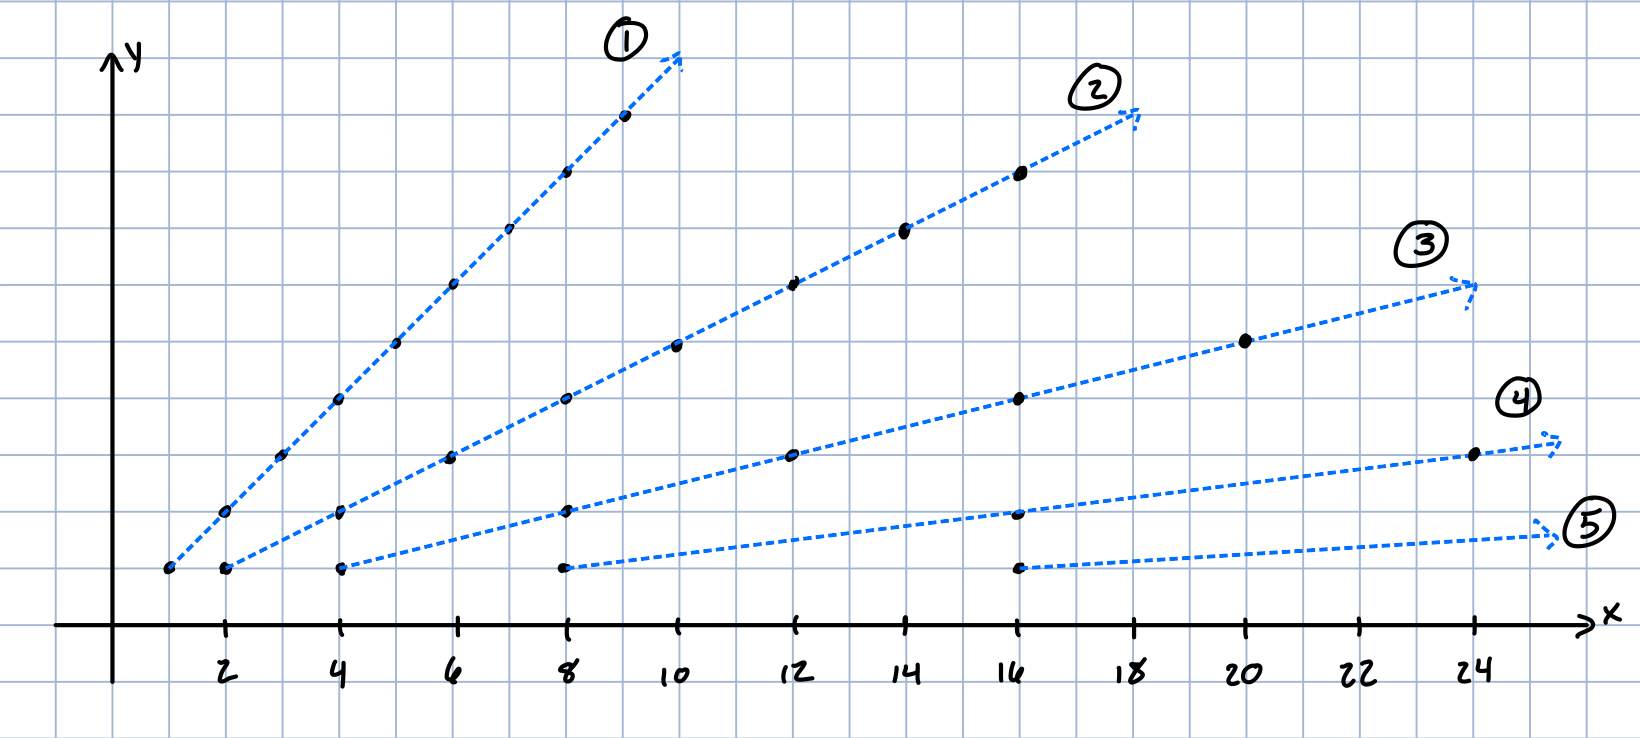
\includegraphics[width=1.0\textwidth]{images/1part2desc.png}
\pagebreak
\question{2}{Let $R$ and $S$ be equivalence relations on a set $A$. Prove or disprove the following statements.}

\part{The relation $R \cup S$ is an equivalence relation on $A$.}
\begin{proof}
	(Counter Example) Suppose $A = \{a, b, c\}$, $R=\{(a,a), (b,b), (c,c), (a,b), (b,a)\}$, and $S=\{(a,a),(b,b),(c,c),(b,c),(c,b)\}$, where $R$ and $S$ are equivalence relations on $A$. Then $R \cup S = \{(a,a),(b,b),(c,c),(a,b),(b,a),(b,c),(c,b)\}$, however, it does not contain $(a,c)$. Therefore, $R \cup S$ is not transitive and not an equivalence relation on $A$.
\end{proof}

\part{The relation $R \cap S$ is an equivalence relation on $A$.}
\begin{proof}
	We must show that $R \cap S$ is reflexive, symmetric, and transitive.
	\begin{enumerate}
		\item Reflexive: Because $R$ and $S$ are each reflexive, then for all $a \in A$, $(a,a) \in R$ and $(a,a) \in S$. This means $(a,a) \in R \cap S$. This shows that $R \cap S$ is reflexive.

		\item Symmetric: Let $(a,b) \in R \cap S$, where $a,b \in A$. This means $(a,b) \in R$ and $(a,b) \in S$, and because $R$ and $S$ are symmetric, $(b,a) \in R$ and $(b,a) \in S$. Therefore, since both relations contain $(b,a)$, then $(b,a) \in R \cap S$. This shows that $R \cap S$ is symmetric.

		\item Transitive: Let $(a,b),(b,c) \in R \cap S$, where $a,b,c \in A$. This means $(a,b),(b,c) \in R$ and $(a,b),(b,c) \in S$. Since $R$ and $S$ are transitive, then $(a,c) \in R$ and $(a,c) \in S$. Therefore, because both relations contain $(a,c)$, then $(a,c) \in R \cap S$. This shows that $R \cap S$ is transitive.
	\end{enumerate}
\end{proof}

\question{3}{The set of integers \textit{modulo n}, where $n > 1$ is a natural number, is denoted $\Z/n\Z$ and is defined as the set of equivalence classes under the equivalence relation on $\Z$ of being congruent modulo $n$. Prove that is it possible to define addition and multiplication operations on $\Z/n\Z$ via the formulas $[a]+[b] = [ a + b]$ and $[a] \cdot [b] = [ a \cdot b]$, respectively.}

\part{Addition: $[a] +[b] = [a+b]$}
\begin{proof}
	Suppose $[a] = [a']$ and $[b]=[b']$, then from this we can say $a = a'+xn$ and $b = b'+yn$, where $x,y \in \Z$. Then, $a+b = a' + b' + n(x + y) \Rightarrow [a+b] = [a'+b']$. To show the existence of identity, $[a] + [0] = [a + 0] = [a]$. Finally, to show the existence of inverse, let's say $[a+(n-a)] = [0]$ which gives us the inverse of $[a]$ being $[n-a]$.
\end{proof}

\pagebreak

\part{Multiplication: $[a]\cdot[b] = [a\cdot b]$}
\begin{proof}
	Suppose $[a]=[a']$ and $[b]=[b']$, then from this we can say $a=a'+xn$ and $b=b'+yn$, where $x,y \in \Z$. Then,
	\begin{align*}
	 	a \cdot b &= (a'+xn) \cdot (b'+yn)\\
	 	a \cdot b &= a'b' + a'yn + b'xn + n^2xy\\
	 	a \cdot b &= a'b' + n(a'y + b'x + nxy).
	 \end{align*}
	 From this, we can then say $[a] \cdot [b] = [a \cdot b]$. To show the existence of identity, $[a]\cdot[1] = [a \cdot 1] = [a]$.
\end{proof}


	
\end{document}